\section{System Overview}
%\section{Star Schema}
%{\bf Star Schema.} 
%{\bf Star schema.} 

Figure~\ref{fig:framework} shows the system diagram for our solution which uses hierarchical intervention. 
The back-end of the system is the spatial data and a spatial database system. 
Users may discover observations by searching the data. Their observations can be generated from data histograms and aggregated queries.
%We take inputs in the form for aggregate queries. An arithmetic expression encapsulates the relationships between these queries. 
The partitioner create a hierarchy partitions on top of spatial data. Depending on the hierarchy that we have created and our inputs, we perform aggravation and intervention. The results of aggravation and intervention are used to in a ranking system based on an explanation index. The explanation index evaluator measures the quality of candidate explanations and outputs the top-k explanations. 
%How much each explanation approach is weighted in the explanation index is under the control of the data analyst. 
%Finally, the top results are used for visualization. We have created a web-based GUI to display these kinds of explanations.

\begin{figure}[t]
	\centering
		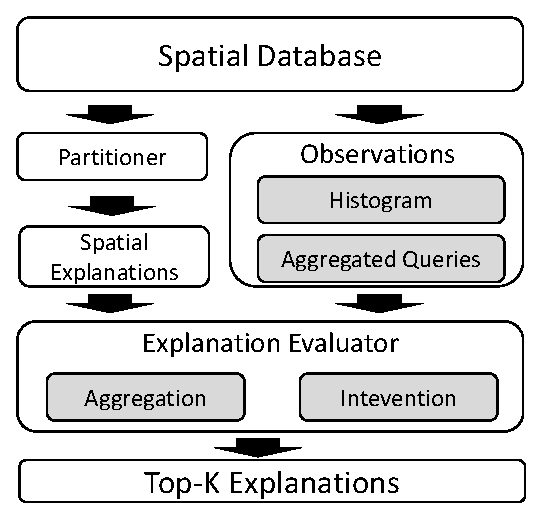
\includegraphics[width=0.4\textwidth]{images/architecture.eps}
		\caption{An outline for our system framework}
	\label{fig:framework}
\end{figure}

The proposed system has the underlying assumption that the data that will be used to generate explanations is the Fact Table for a Star schema\cite{giovinazzo2000object,adamson2010star}. To understand the Fact Table, it is important to understand the structure of the Star Schema. A traditional relational database system contains a set of tables related by primary and foreign keys. For instance, we can use our running example of the NYC Taxi Trips dataset to illustrate a Star Schema. The trips and payment type can be represented in separate tables. One trip can have a single payment type while a payment type can be used in multiple trips. This is an example of a one-to-many relationship.
In order to represent this data in a relational database, the $trips$ table and the $payment\_type$ table need to have a primary and foreign key. Table~\ref{tbl:fact} can be considered as the central part of the schema because it contains the foreign key to the $payment\_type$ table.



% \begin{center}
% \small
%   \begin{tabular}{ | l | c | }
%     \hline
%     \textbf{PaymentTypeId} & \textbf{Name} \\ \hline
%     1 & Credit Card  \\ \hline
%     2 & Cash  \\ \hline
%     3 & No Charge  \\
%     \hline
%   \end{tabular}
% \end{center}
% \captionof{table}{Payment Type Table}
% \label{tbl:payment_type}

% \begin{center}
%   \begin{tabular}{ | l | c | r | }
%     \hline
%     \textbf{StudentId} & \textbf{Name} & \textbf{Grade} \\ \hline
%     1 & John Doe & 3.2 \\ \hline
%     2 & Alice & 3.3 \\ \hline
%     3 & Bob & 3.8 \\
%     \hline
%   \end{tabular}
% \end{center}
% \captionof{table}{Students Table}
% \label{tbl:student}

\begin{center}
\small
  \begin{tabular}{ | l | l | c | l | }
    \hline
    \textbf{pickup\_lat} & \textbf{pickup\_lng} & \textbf{PaymentType} & \textbf{tip\_percentage} \\ \hline
    34.4 & -74.2 & 1 & 15.3 \\ \hline
    34.6 & -74.1 & 1 & 10.2 \\ \hline
    34.6 & -74.3 & 1 & 9.8 \\ \hline
    34.8 & -74.6 & 2 & 11.2 \\ \hline
    34.6 & -74.3 & 1 & 10.7 \\ \hline
    34.9 & -74.1 & 3 & 0.0 \\
    \hline
  \end{tabular}
\end{center}
\captionof{table}{\small Trips Table. PaymentType 1, 2, and 4 represent Credit Card, Cash, and No Charge, respectively.}
\label{tbl:fact}

This type of schema where there is a central table consisting of facts while the remaining tables contain the meta data is called a star schema. The central table is called the Fact Table, whereas, the tables containing the meta data are called the Dimension Tables (such as the payment type table in the NYC Taxi Trip dataset).% In the case of the schema we just defined, Table.~\ref{tbl:payment_type} is the dimension table while Table.~\ref{tbl:fact} is the fact table.

%\section{Observations}
% \begin{figure}[ht]
%   \begin{center}
%   \includegraphics[width=0.5\columnwidth]{observationexample}
%   \end{center}

%   \caption{An histogram showing an example observation}
%   \label{fig:observation_example}
% \end{figure}

{\bf Numeric Query.} A numeric query is an expression of the form:
$$Q = E(q_1, q_2, .., q_m)$$
Here $q_i$ is any SQL query which contains an aggregate function. The aggregate function can be SUM, COUNT, and AVERAGE. So each $q_i$ will return a single numeric value. $E$ represents a numeric expression based on the result of $q_1$, $q_2$, .., $q_m$. The operator in $E$ can be any numeric operator, such as $+$, $-$, $*$, $/$, $log$, etc.

{\bf {\Fact}.} A {\fact} is a pair $(Q, dir)$, where (1) $Q$ is a numeric query, (2) $dir \in \{high, low\}$ is direction indicating whether the user thinks $Q$ is higher or lower than the expected value.

{\bf Example.} In Figure \ref{fig:spatial_explanation_example}, there a {\fact} that the number of taxi trips in NYC on January 23, 2016 dropped drastically. Such {\fact} can be represented by two queries, $q_1$ and $q_2$ as follows:

\renewcommand{\lstlistingname}{Query}% Listing -> Algorithm
\begin{lstlisting}[language=SQL, caption=Aggregate Query for the number of taxi trips on January 22, label=qry:aggregateexample1]
SELECT COUNT(*) FROM
FROM nyc_data
WHERE date = 'January 22, 2016'
\end{lstlisting}
\renewcommand{\lstlistingname}{Query}% Listing -> Algorithm
\begin{lstlisting}[language=SQL, caption=Aggregate Query for the number of taxi trips on January 23, label=qry:aggregateexample2]
SELECT COUNT(*) FROM
FROM nyc_data
WHERE date = 'January 23, 2016'
\end{lstlisting}
The difference in the number of taxi trips between the two dates can be represented by a numeric query $Q = \frac{q_1}{q_2}$. The number of taxi trips drops drastically, so it means the value of $Q$ is lower than the expected value. Then the {\fact} has the format $(\frac{q_1}{q_2}, low)$.

When a table is analyzed, users may find an interesting {\fact} from the data table. This {\fact} is issued to the system with the defined format as the input. Then the system will try to find out the {\explanation} for the {\fact}.

%{\bf {\Fact}s.} {\Fact}s are features in the data that the user wants to explain. {\Fact}s are defined as arithmetic expressions over a set of aggregate queries. Let $F$ be the fact table in our star schema dataset. In the course of this document, we will be using relational algebra expressions defined by \cite{elmasri2011fundamentals} for aggregate expressions. Thus, the $\mathscr{F}$ symbol represents an aggregate function. An aggregate query is defined as:
%$$_A\mathscr{F}_B(D), A \in F$$
%$B$ is an aggregate function. $A$ is an attribute in our dataset. $D$ is the fact table. Examples of an aggregate function include SUM, COUNT, and AVERAGE.
%We use SQL to construct an example for an observation. Queries~\ref{qry:aggregateexample1} and \ref{qry:aggregateexample2} show examples of aggregate queries.

% Observations made on data can also be represented on histograms. Fig.~\ref{fig:observation_example} shows an example of an observation. The green bar on the histogram represents an aggregate query where the day is Friday.

%\renewcommand{\lstlistingname}{Query}% Listing -> Algorithm
%\begin{lstlisting}[language=SQL, caption=Aggregate Query for average tip percentage with credit cards, label=qry:aggregateexample1]
%SELECT AVG(tip_percentage) FROM
%FROM nyc_data
%WHERE payment_type = 1
%\end{lstlisting}
%\renewcommand{\lstlistingname}{Query}% Listing -> Algorithm
%\begin{lstlisting}[language=SQL, caption=Aggregate Query for average tip percentage with cash, label=qry:aggregateexample2]
%SELECT AVG(tip_percentage) FROM
%FROM nyc_data
%WHERE payment_type = 2
%\end{lstlisting}

%Using these aggregate queries we may form an observation based on the ratio of tip percentage with credit card against tip percentage with cash.
%$$observation = \frac{\textnormal{Query.~\ref{qry:aggregateexample1}}}{\textnormal{Query.~\ref{qry:aggregateexample2}}}$$


%\section{Explanations}
{\bf {\Explanation}.} We represent an {\explanation} as a predicate $\phi$. 
A predicate $\phi$ is a conditional statement which results in a boolean value. An {\explanation} indicates a set of tuples in the data table which satisfy the predicate. For non-spatial {\explanation}, $\phi$ has the format of $[A$ $op$ $c]$, where $A$ is an attribute in the data table, $op$ can be $=$, $<$, $\leq$, $>$, $\leq$ and $c$ is a numeric value. For example, we can have an non-spatial {\explanation} as follows:
$$\phi: PaymentType = 1$$
If we use such {\explanation} to explain the {\fact} mentioned previously, it means we think that the drop on 22 January, 2016 is caused by the trips which are paid by Type 1 (but actually this explanation does not make sense).

%We go into more details for the formal definition of different kinds of explanations in Section~\ref{sec:taxonomy}. 
%If we consider Queries~\ref{qry:aggregateexample1} and \ref{qry:aggregateexample2} as an example. The explanation would be in the form of a predicate:
%$$tip\_percentage = 15.3$$
%
%Let $D$ be our solution space. We can define our predicate to be the function $P$. Let $X$ represent a set of attributes in our schema. Our explanation can now be formally defined as:
%
%\begin{equation}
%X|P(X):=
%    \begin{cases}
%      \text{true}, & \text{if}\ X \in D \\
%      \text{false}, & \text{otherwise}
%    \end{cases}
%\end{equation}

%Note that $P$ is an open ended function. In the case of spatial explanations, $P$ can take the form of a spatial function like $ST\_CONTAINS$ in PostGIS i.e. whether a polygon contains a point. In the non spatial context, $P$ can represent functions like 'greater than', 'less than', etc.


{\bf {Explanation via Intervention.}} 
%\my{Intervention is an approach inspired by the concept of influence. It builds on the \my{aggravation} approach(Section~\ref{sec:aggravation}).}  
The Intervention approach measures how much the {\fact} would change had the explanation not been present. Let $D$ be the dataset we are interested in and $Q$ be a function which returns the value of our target {\fact} given a dataset. Keeping our taxonomy in context, this means $Q$ returns the value of our aggregate {\fact} query. Denote $\phi$ as one candidate {\explanation}. Let $\Delta_\phi \leftarrow \sigma_\phi(D)$ be a subset of $D$ that satisfy $\phi$. Then $D - \Delta_\phi$ represents the remaining part after removing $\Delta_\phi$ from $D$. The direction of the {\fact} can either be \textit{high} or \textit{low} depending on whether we are interested in the greatest or least values of {\fact} respectively. Given a dataset $D$, a {\fact}$(Q, dir)$, the degree of an {\explanation} $\phi$ by intervention can be defined as follows:
\begin{equation}
\delta_{int}:=
\begin{cases}
-Q(D-D_{\phi}), & \text{if}\ direction=high \\
Q(D-D_{\phi}), & \text{otherwise}
\end{cases}
\end{equation}

The degree of candidate explanation by intervention must be higher the closer we are to the direction of the observation, therefore, we use the negative value when the direction is high. If the influence of the candidate explanation is high, it will result in a low observation value once the candidate explanation is removed from the dataset.
Since intervention extends the idea presented by aggravation, it has similar issues when it comes to the number of permutations for candidate explanations. Similar to our approach in aggravation(Section~\ref{sec:aggravation}), we can reduce the number of permutations by \my{bucketing} the attributes. We can extend intervention for spatial observations and explanations the same way we did for aggravation. The set $P$ consists of distinct non overlapping polygons in our dataset $D$. Let $s$,$t$ be the spatial attributes in $D$. \my{Each tuple in $P$ has two attributes: $polygon\_id$, and $polygon$.}


{\bf Finding Spatial Explanations.}
%{\bf Spatial {\Explanation}.} 
A spatial {\explanation} is different that general {\explanation} in that it is represented by a spatial predicate. A spatial {\explanation} actually indicates a set of data tuples that can satisfy the spatial predicate. We denote a spatial {\explanation} as $\phi_S$.
Spatial explanations take the spatial attributes of the data into consideration. In contrast to non spatial explanations, the candidate spatial explanations consists of polygons. Since we base our proposed approach on the assumption that important tuples are spatially co-located, points which fall inside these polygons form a candidate explanation. 
%Let $S$ be the spatial attributes of $D$ and $P$ be the set of all possible polygons that can be formed from $S$. Let $G$ be a function such that$G(s,t)$ is true when $(s,t) \in P$ and false otherwise, where $s$,$t$ are the dimensions of a point in the Cartesian plane. Our candidate explanation can be defined as,
%$$\phi  \models \vee_{l,k} G(l,k)$$
%where $k,l \in A_D$

%\my{This example should be modified because it looks like a non-spatial explanation.}
%To illustrate spatial explanation in action, we can use NYC TLC data again. Fig.~\ref{fig:spatial_explanation_example} shows the explanation in terms of tip percentage where the observation is also the average tip percentage.

%\begin{figure}[ht]
%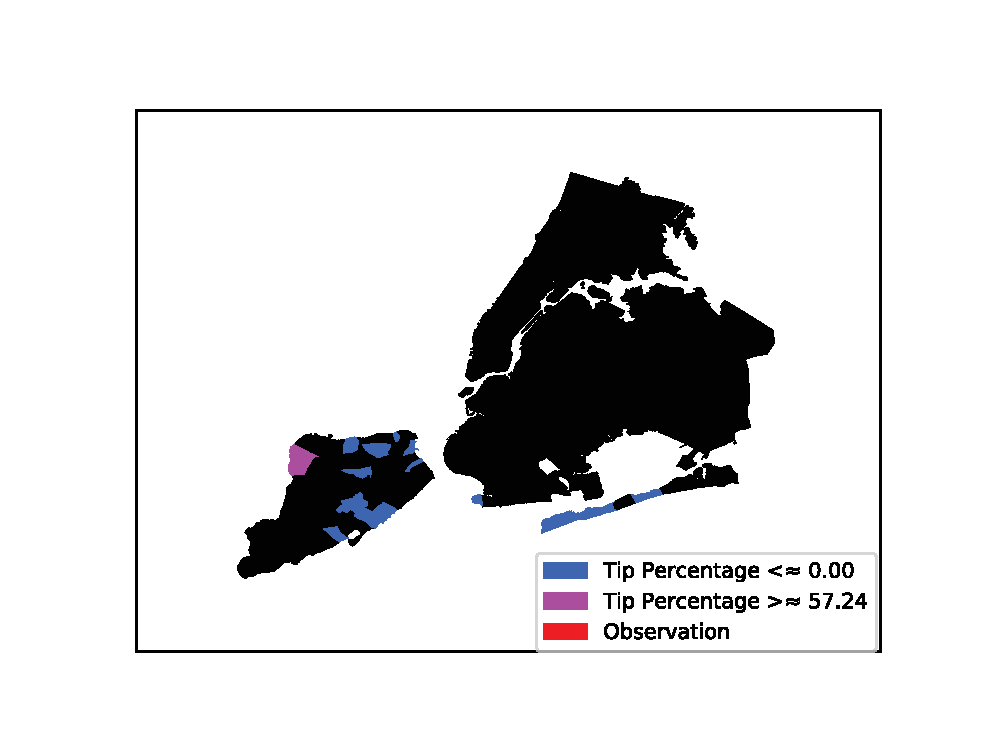
\includegraphics[width=\columnwidth]{images/spatial_explanation_example.eps}
%\caption{An example of spatial explanation}
%\label{fig:spatial_explanation_example}
%\end{figure}

The polygons painted purple show polygons in the candidate {\explanation} where the tip percentage is high, while polygons painted blue show candidate explanations where the tip percentage is low. It should be noted that $P$ has a high number of permutations. It is up to the approach to decide which polygons to include in the candidate explanation. For instance, hierarchical intervention may choose polygons in a spatial proximity while aggravation may choose otherwise.
\begin{figure}[t]
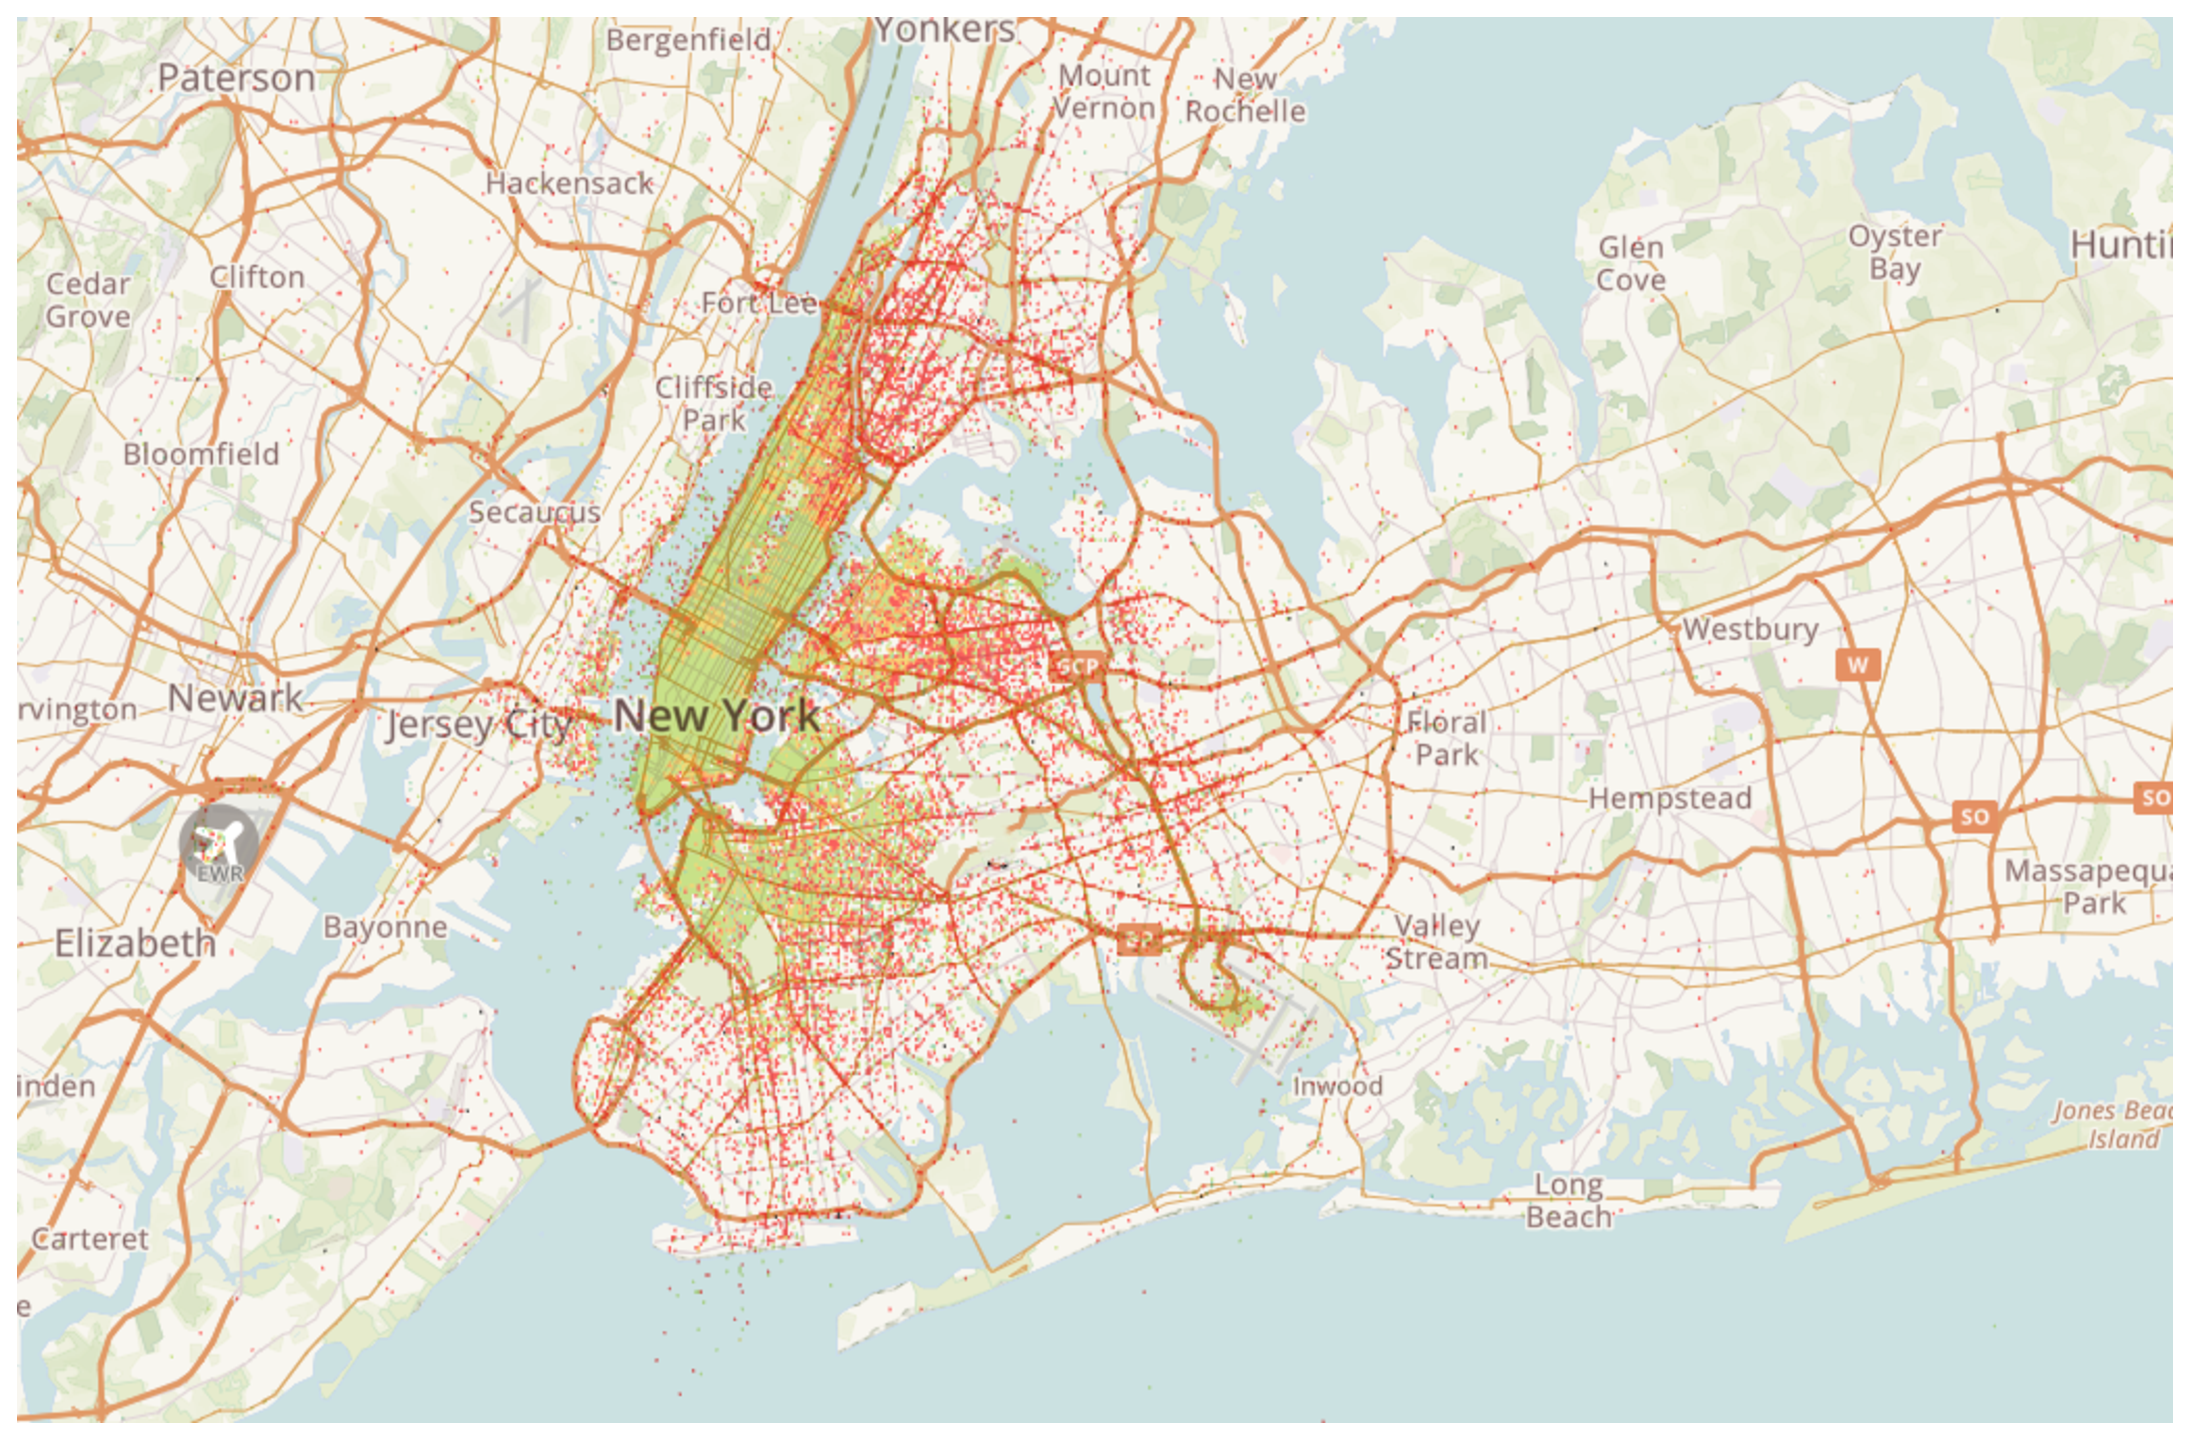
\includegraphics[width=\columnwidth]{images/scatter}
\caption{Heatmap for NYC trips for January 2016}
\label{fig:square_unit_grid}
\end{figure}

\my{Another interesting consideration when we are talking about spatial explanations is the density of the data. Fig.~\ref{fig:square_unit_grid} shows the heatmap for tip percentage with respect to pickup coordinates. It is interesting to observe that the explanations provided in Fig.~\ref{fig:spatial_explanation_example} are all areas with low density of data. One of the reasons for this is because each approach takes some liberty with our definition of the taxonomy. Even though, we defined $P$ to contain all permutations of polygons, an approach may use limited polygons, such as neighborhoods or zones. The way the explanation is ranked also plays a large role.}




% \section{Front End Visualization Tools}
% React\cite{reactjs} is a front end framework which originated in Facebook. The React framework allows interfaces to be designed using components. Each component has properties and a state. A component can have subcomponents. This makes it simpler to design interfaces which show consistent data across components. Some of the charts included in the interface make use of the eCharts library\cite{echarts}.

% MapBox\cite{mapbox} is a library for displaying maps. The maps provided by mapbox consists of tiles and vectors. Each tile represents a cube of the map while vectors are shapes which represent roads, buildings, etc. Deck.gl\cite{deckgl} is a library for creating an overlay on top of the map. Examples of overlays include scatterplots, cartograms etc. Matplotlib was also used for static plots for evaluation\cite{hunter2007matplotlib}.

% We have used all of these tools in a GUI for our our framework. The details of the implementation can be found in Section~\ref{sec:implementation}
